\chapter{ADVANCED AI PROJECTS}

This chapter describes the transition from traditional machine learning projects to advanced computer vision and industrial AI applications. It details how the foundational concepts acquired in the previous weeks were applied to develop complex, real-world AI systems.

\section{Smart Cam Classifier}

The Smart Cam Classifier project served as a comprehensive introduction to the complete workflow of image classification, utilizing Google's Teachable Machine platform and Python Streamlit. 

\textbf{Introduction:} Image classification is a core application of modern Artificial Intelligence, enabling systems to automatically categorize images into predefined classes. It relies on deep neural networks to learn visual features, such as edges, textures, and shapes, from labeled datasets.

\textbf{Objective:} The primary objective of this project was to develop an AI-powered image classification system capable of identifying different object categories from uploaded images, serving as a practical introduction to computer vision and the deployment of trained machine learning models.

\subsection{Dataset Preparation}

The preparation of high-quality datasets is critical in computer vision. The project emphasized the concept of \textbf{Garbage In, Garbage Out (GIGO)}, illustrating that poor-quality or biased datasets inevitably produce inaccurate AI models.

To ensure robustness, images were collected with extreme care, ensuring diversity in:
\begin{itemize}[leftmargin=1.5cm]
    \item Different backgrounds
    \item Varying lighting conditions
    \item Multiple camera angles
    \item Different orientations
\end{itemize}

Dataset balancing was performed to ensure that each class had an equal representation of images, preventing the model from developing a bias toward a majority class. This diversity ensures that the model generalizes well to unseen data.

\subsection{Model Training and Export}

Training was conducted using \cite{google_teachable} Google Teachable Machine. The process involved creating distinct classes, uploading the curated images, and initiating the training process. During validation, prediction confidence and model accuracy were closely monitored to prevent overfitting and ensure proper generalization. The trained model successfully learned to extract relevant image features automatically.

Upon successful training, the model was exported in the TensorFlow/Keras format. This export process generated two vital files: \texttt{keras\_model.h5}, containing the trained neural network weights, and \texttt{labels.txt}, containing the class definitions.

\subsection{Streamlit Deployment and User Interface}

The deployment application was developed using Python, \cite{tensorflow} TensorFlow, Streamlit, NumPy, and the Pillow library for image processing.

The application pipeline involved:
\begin{enumerate}[leftmargin=1.5cm]
    \item Accepting image uploads from the user.
    \item Resizing the images to match the model's expected input dimensions.
    \item Converting the image to RGB format and normalizing the pixel values.
    \item Passing the processed image to the prediction pipeline.
    \item Displaying the prediction alongside a confidence score.
\end{enumerate}

The user interface was significantly enhanced to feature a responsive layout, modern prediction cards, dynamic confidence bars, and a professional dashboard layout. Explorations into \cite{google_stitch} Google Stitch provided inspiration for modern UI design, prompting discussions on migrating the application from Streamlit to a more flexible Flask architecture.

\subsection{Challenges and Debugging}

A major challenge encountered during deployment was a TensorFlow compatibility issue. Version conflicts between legacy Keras models exported by Teachable Machine and newer TensorFlow installations caused model loading failures. Through a rigorous debugging methodology, the issue was resolved by utilizing the \texttt{tf\_keras} compatibility package, which successfully facilitated model deserialization.

\subsection{Project Outcome}

The Smart Cam Classifier project successfully demonstrated the practical application of Computer Vision and Image Classification. It provided vital experience in TensorFlow deployment, dependency debugging, and application development, serving as the perfect transition toward the highly complex industrial AI project that followed.

\begin{figure}[H]
\centering
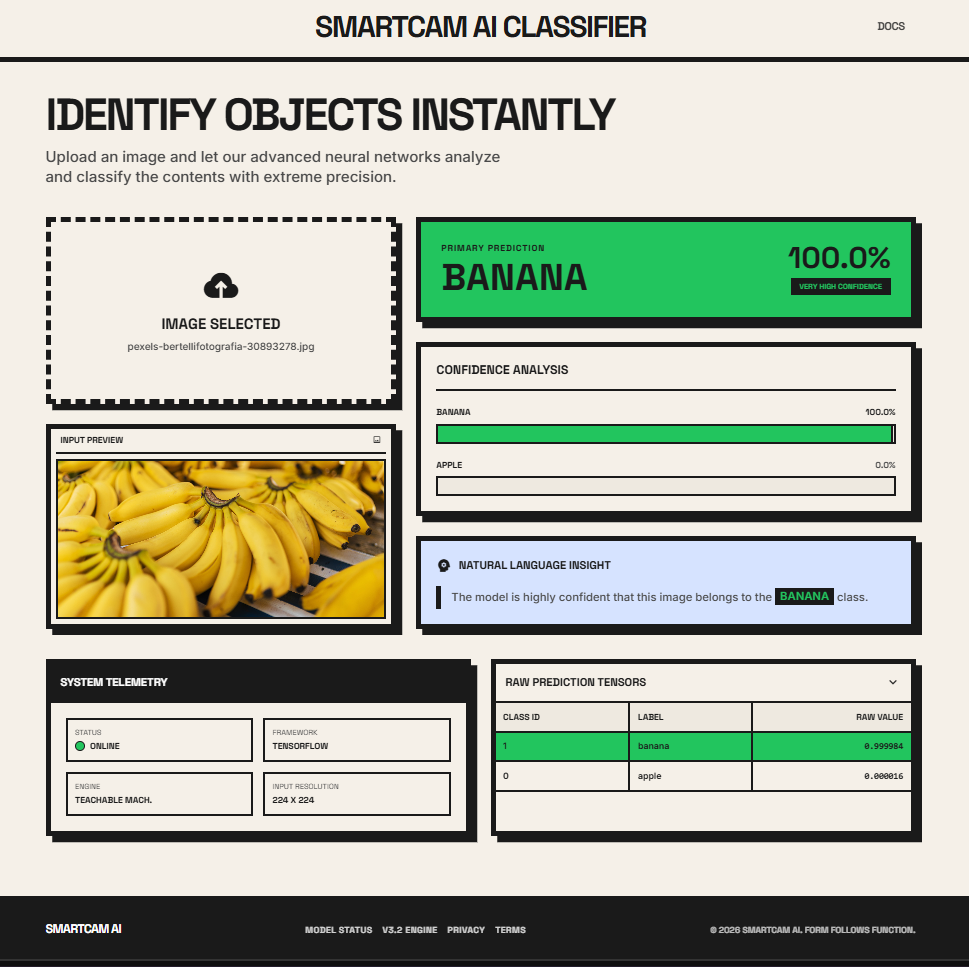
\includegraphics[width=0.7\textwidth]{images/smart_cam_classifier.png}
\caption{Smart Cam Classifier Prediction Interface}
\label{fig:smart_cam}
\end{figure}

\section{QualiVision AI – AI Based Live Tomato Freshness Detection System}

This final capstone project represents the culmination of the internship, applying all accumulated knowledge into a single, enterprise-grade application.

\subsection{Introduction}

Industrial Quality Control traditionally relies on human inspection to identify defective products on manufacturing and sorting lines. However, manual inspection is notoriously slow, inconsistent, labor-intensive, and prone to error due to visual fatigue. Artificial Intelligence and Computer Vision offer modern alternatives, capable of inspecting items continuously with high accuracy and speed. QualiVision AI was motivated by the need to develop an automated quality inspection system for the food industry.

\subsection{Problem Statement}

Food processing industries require fast, reliable, and automated quality inspection systems. The physical throughput of conveyor belts often exceeds the capacity of human inspectors. The objective of this project was to automate the quality inspection of tomatoes (categorizing them as fresh or rotten) using deep learning, thereby reducing operational costs and increasing consistency.

\subsection{Objectives}

The specific objectives of QualiVision AI included:
\begin{itemize}[leftmargin=1.5cm]
    \item Developing an Automatic Image Classification model for real-time prediction.
    \item Designing an Industrial Dashboard for live system monitoring.
    \item Maintaining a Prediction History through robust database integration.
    \item Implementing Explainable AI to visually justify model predictions.
    \item Enabling automated Report Generation for production managers.
    \item Successfully deploying the system via a web architecture.
\end{itemize}

\subsection{System Overview}

The complete system workflow is designed for efficiency and traceability:
Image Acquisition $\rightarrow$ Image Preprocessing $\rightarrow$ Deep Learning Model $\rightarrow$ Prediction $\rightarrow$ Confidence Score $\rightarrow$ Grad-CAM Visualization $\rightarrow$ Database Storage $\rightarrow$ Dashboard Display $\rightarrow$ Reports.

\begin{figure}[H]
\centering
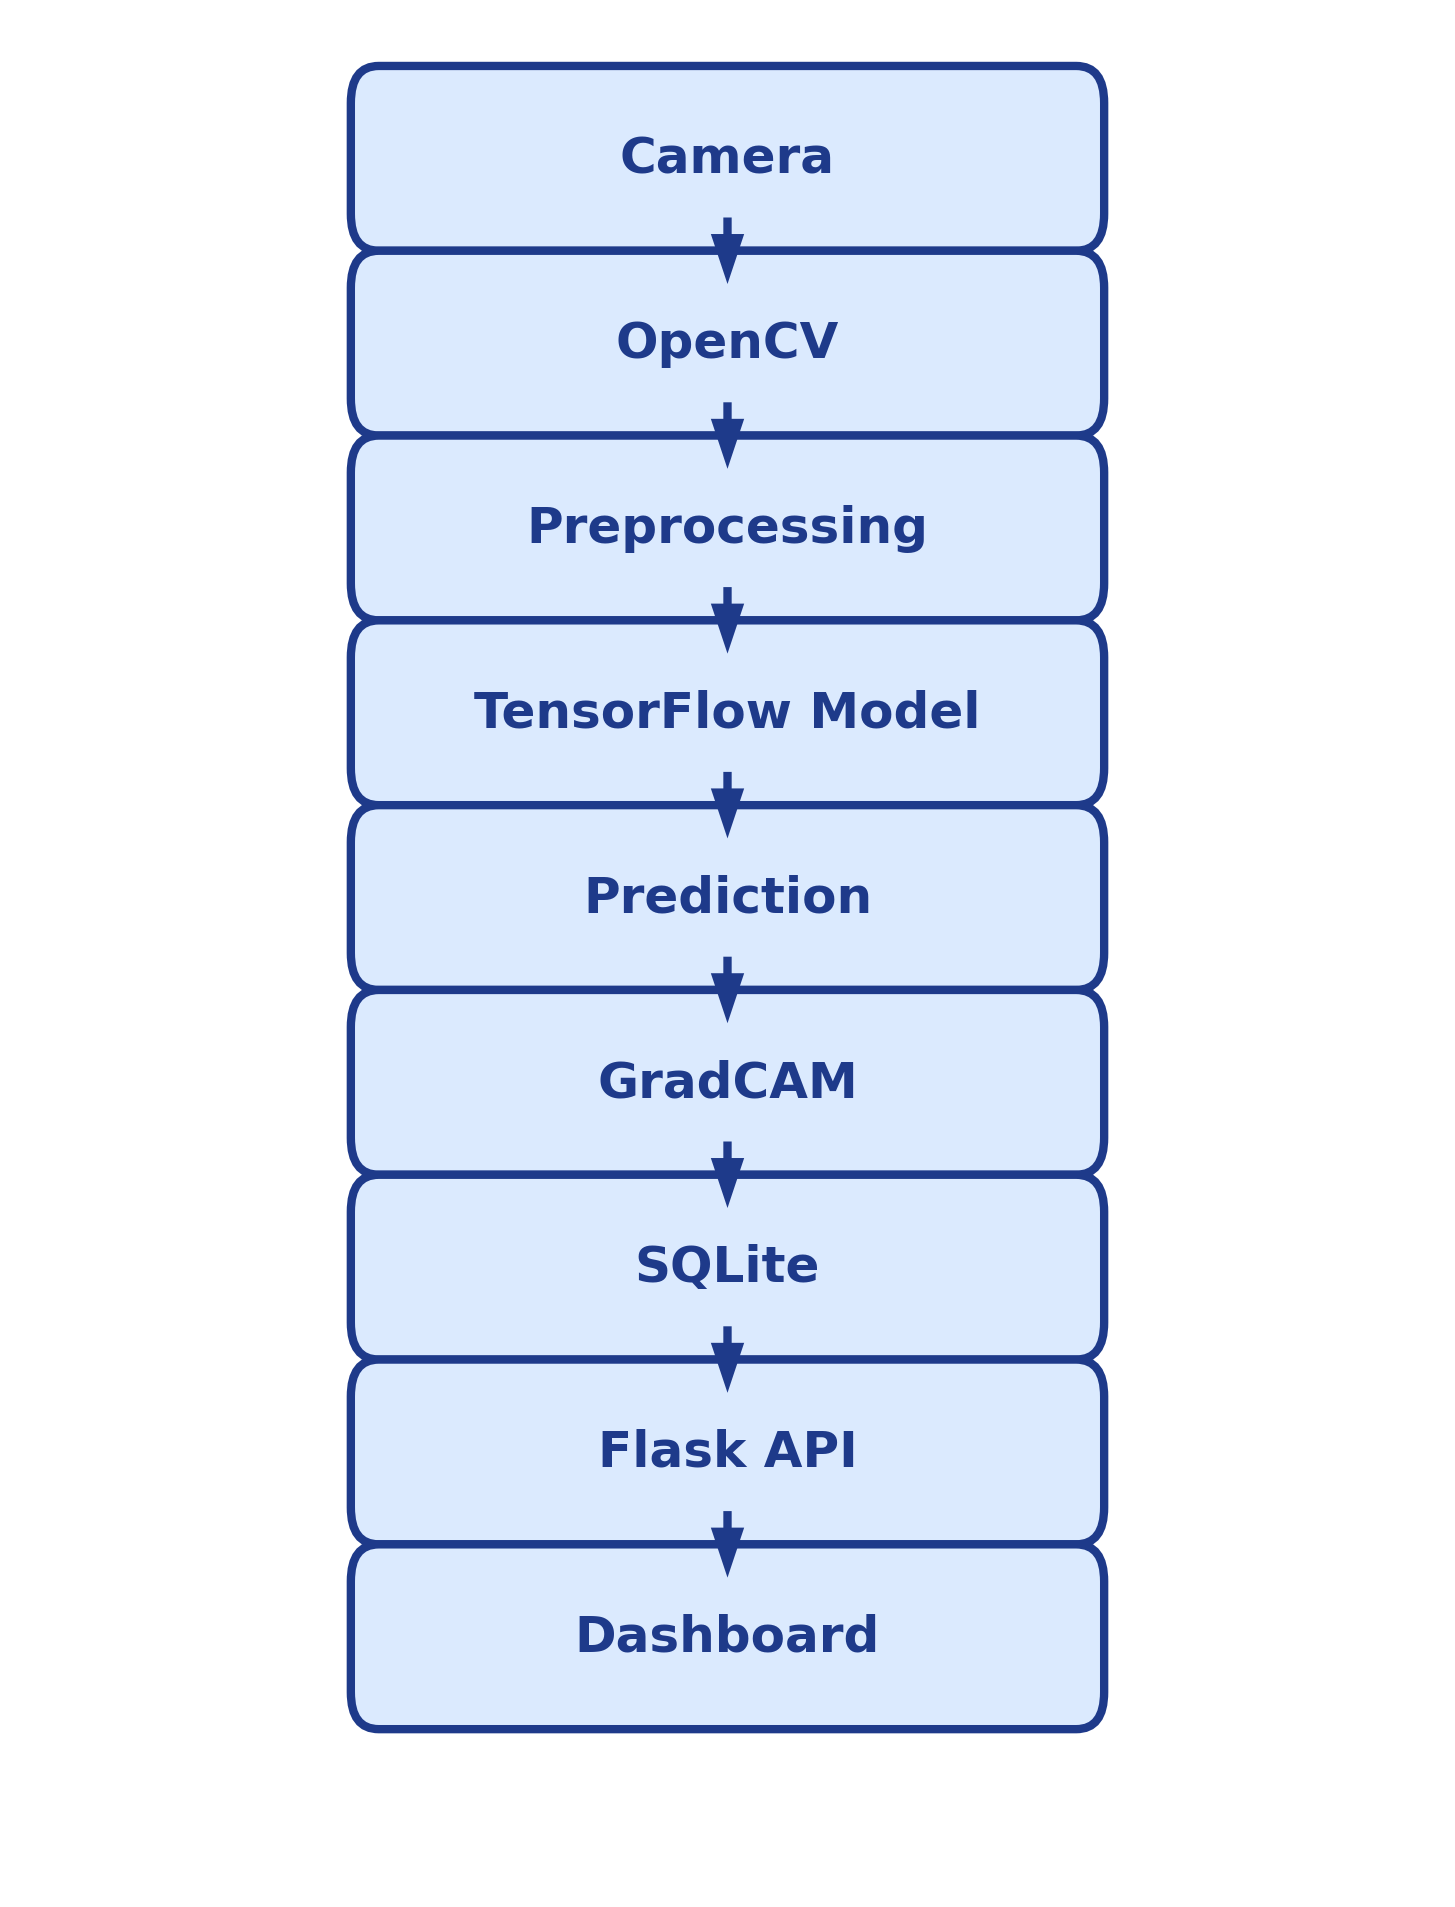
\includegraphics[width=0.8\textwidth]{images/architecture.png}
\caption{System Architecture of QualiVision AI}
\label{fig:qualivision_arch}
\end{figure}

\subsection{Dataset and Preprocessing}

Dataset collection involved sourcing high-quality images from public datasets such as Kaggle. The images were meticulously organized into `Fresh Tomatoes` and `Rotten Tomatoes` categories. Extensive cleaning was performed to remove duplicates and irrelevant images, ensuring dataset balancing across the training, validation, and testing splits. The project reinforced that dataset quality directly dictates model accuracy.

Academically rigorous image preprocessing was applied before training, including:
\begin{itemize}[leftmargin=1.5cm]
    \item Image Resizing to standard dimensions.
    \item RGB Conversion.
    \item Normalization of pixel values.
    \item Data Augmentation to introduce variability and prevent overfitting.
    \item Batch Processing for efficient memory utilization.
\end{itemize}

\subsection{Transfer Learning and Model Training}

The project utilized Transfer Learning with the \textbf{EfficientNetV2B0} architecture. Pretrained on millions of images, this model was selected for its exceptional balance of high accuracy and low training time, making it ideal for edge deployment.

The model training pipeline was developed using TensorFlow and \cite{keras} Keras. Training parameters were carefully tuned, including Batch Size, Epochs, Learning Rate, Adam Optimizer, and Binary Crossentropy Loss Function. Advanced techniques such as Early Stopping and Learning Rate Schedulers were employed to optimize convergence during validation.

\begin{figure}[H]
\centering
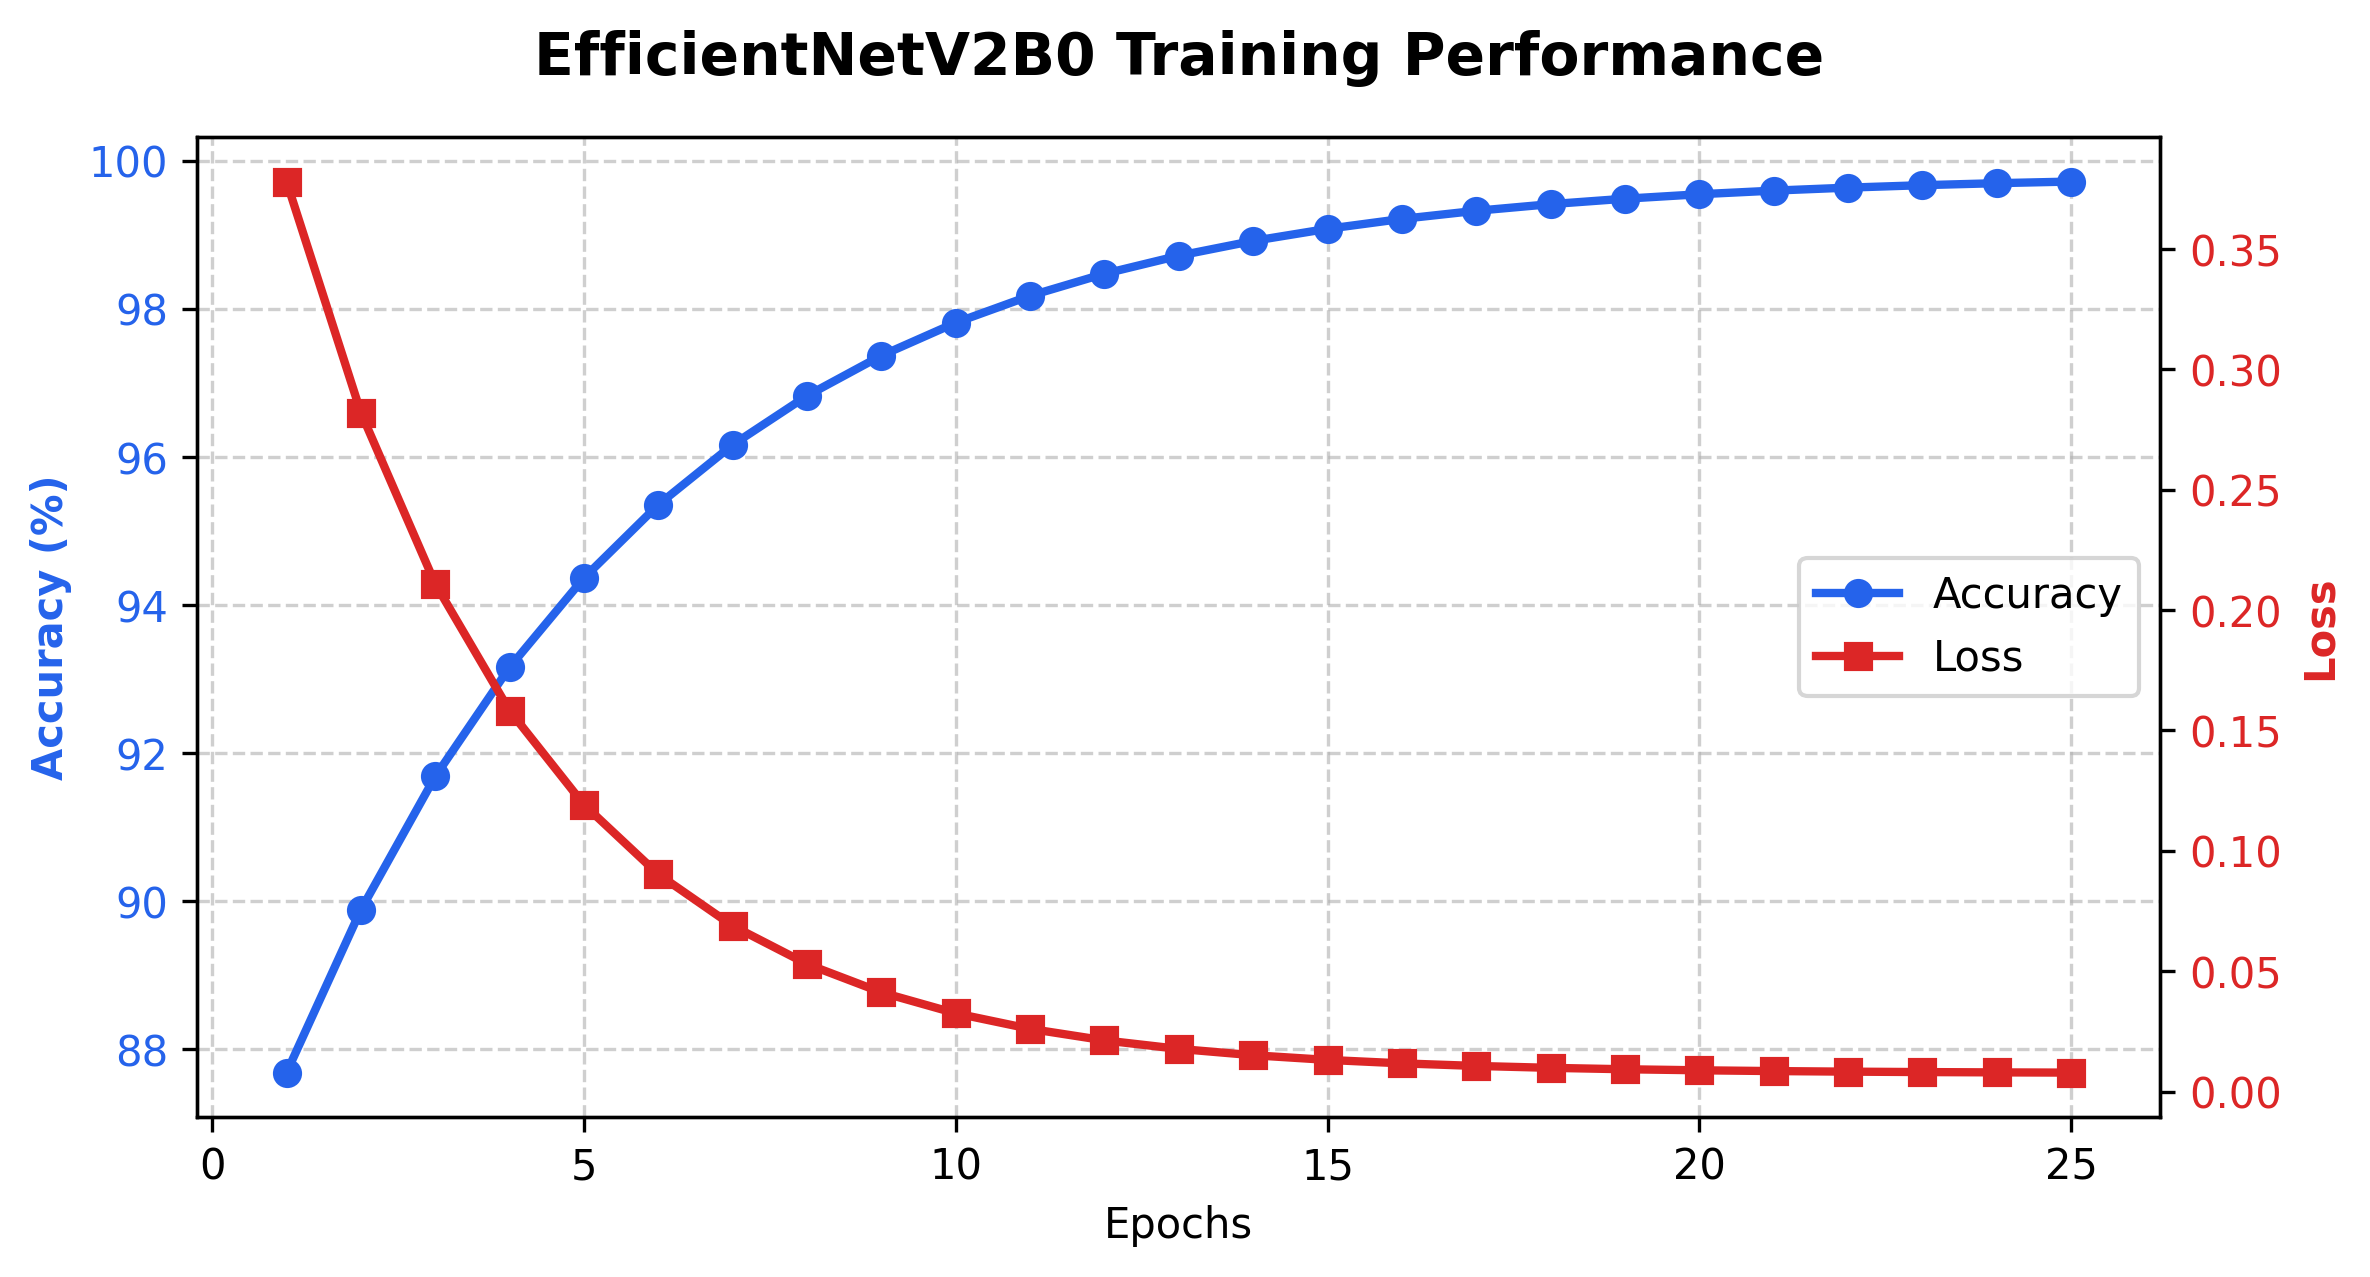
\includegraphics[width=0.8\textwidth]{images/performance_chart.png}
\caption{Model Training Performance}
\label{fig:training_curves}
\end{figure}

\subsection{Model Evaluation and Explainable AI (Grad-CAM)}

The model was rigorously evaluated using standard metrics, including Accuracy, Precision, Recall, and F1 Score. The Confusion Matrix and Classification Report provided granular insights into false positives and false negatives, while the ROC Curve illustrated the model's discriminative ability based on prediction confidence.

To ensure trust in the automated system, Explainable AI was integrated. Gradient-weighted Class Activation Mapping (\textbf{Grad-CAM}) was implemented to visualize the specific regions of the image that strongly influenced the model's prediction. This is critical in industrial AI, as operators must understand \textit{why} a product was rejected.

\begin{figure}[H]
\centering
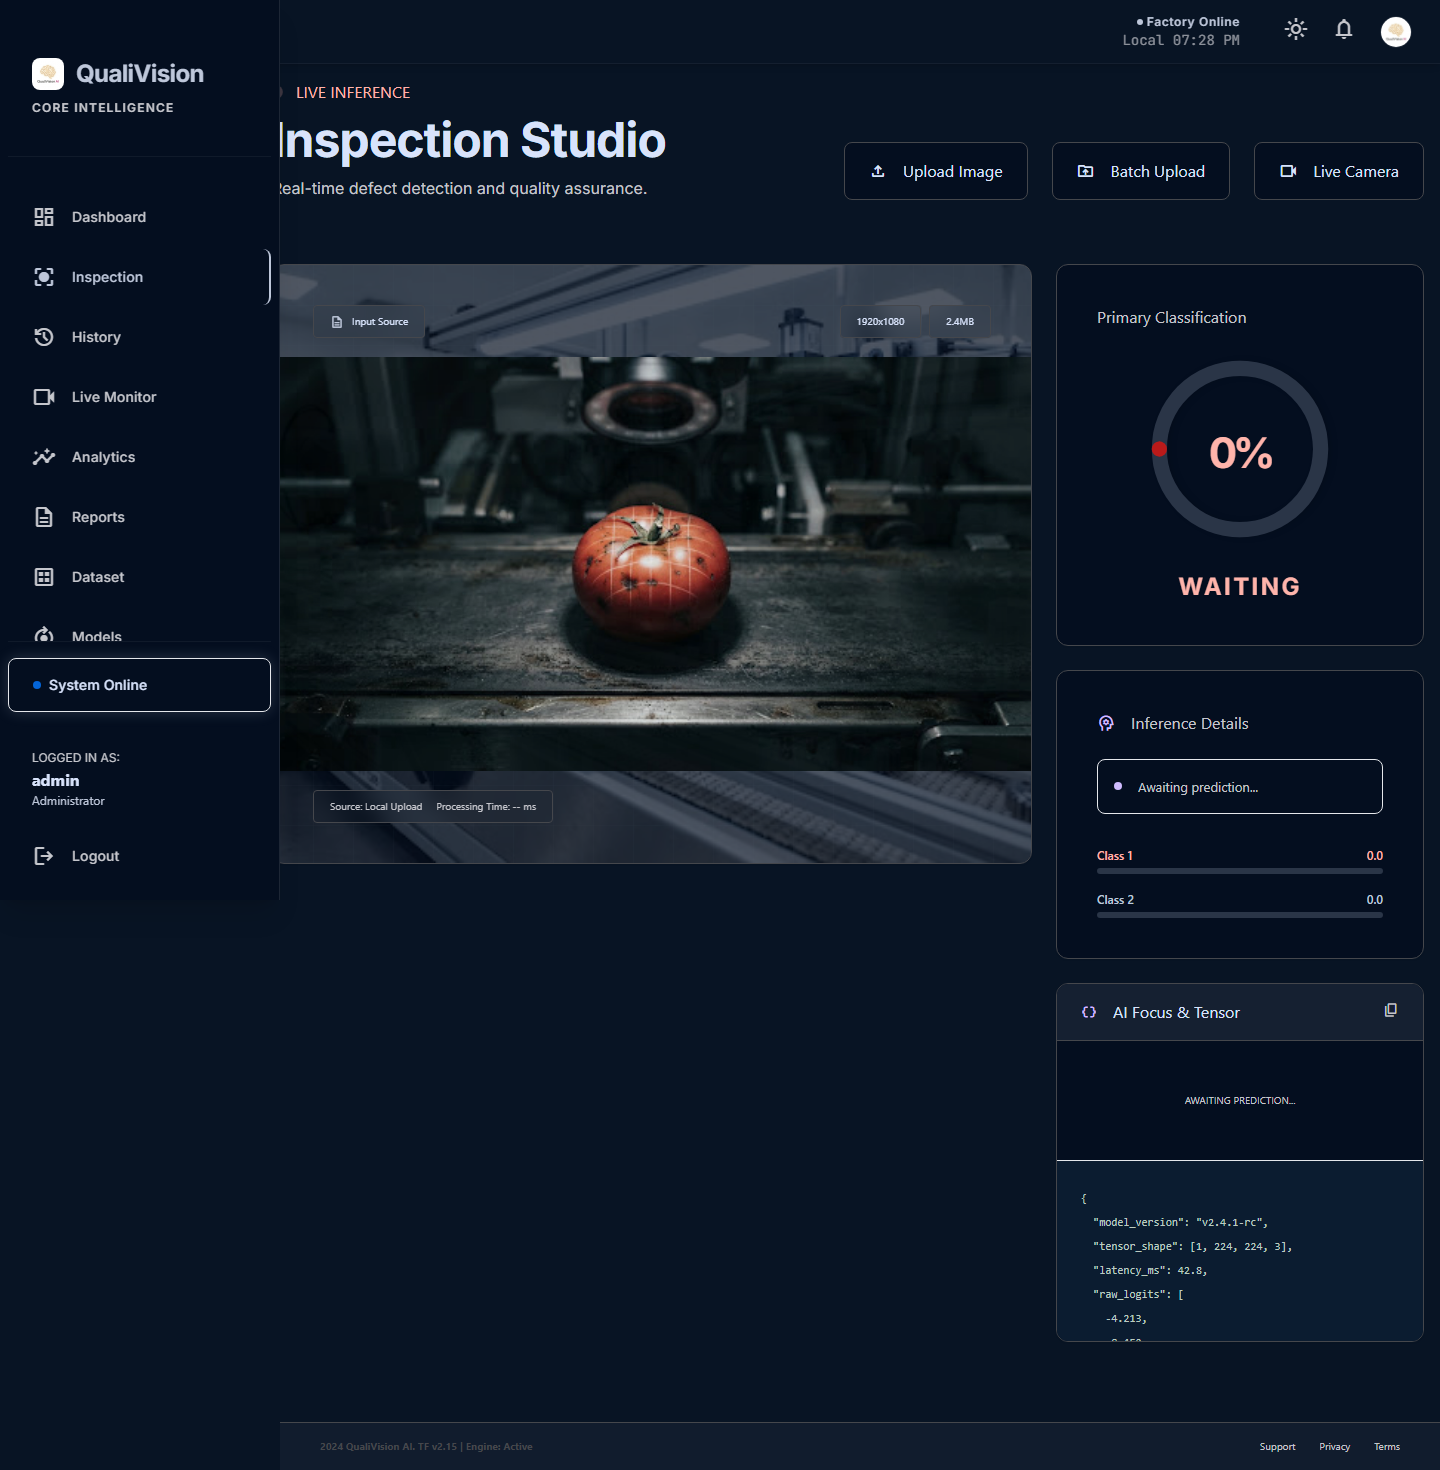
\includegraphics[width=0.8\textwidth]{images/04-inspection.png}
\caption{Grad-CAM Visualization on Defective Produce}
\label{fig:gradcam}
\end{figure}

\subsection{Backend Development and Database}

The backend architecture was developed using the \cite{flask} Flask framework, organized using Blueprints for modularity. REST APIs were developed to handle core services, including Prediction APIs, Dashboard APIs, History APIs, and Report APIs.

SQLite was integrated to ensure persistent storage of inspection records. The database logs the Prediction, Timestamp, Confidence Score, Image Path, and Status of every inspected item.

\begin{figure}[H]
\centering
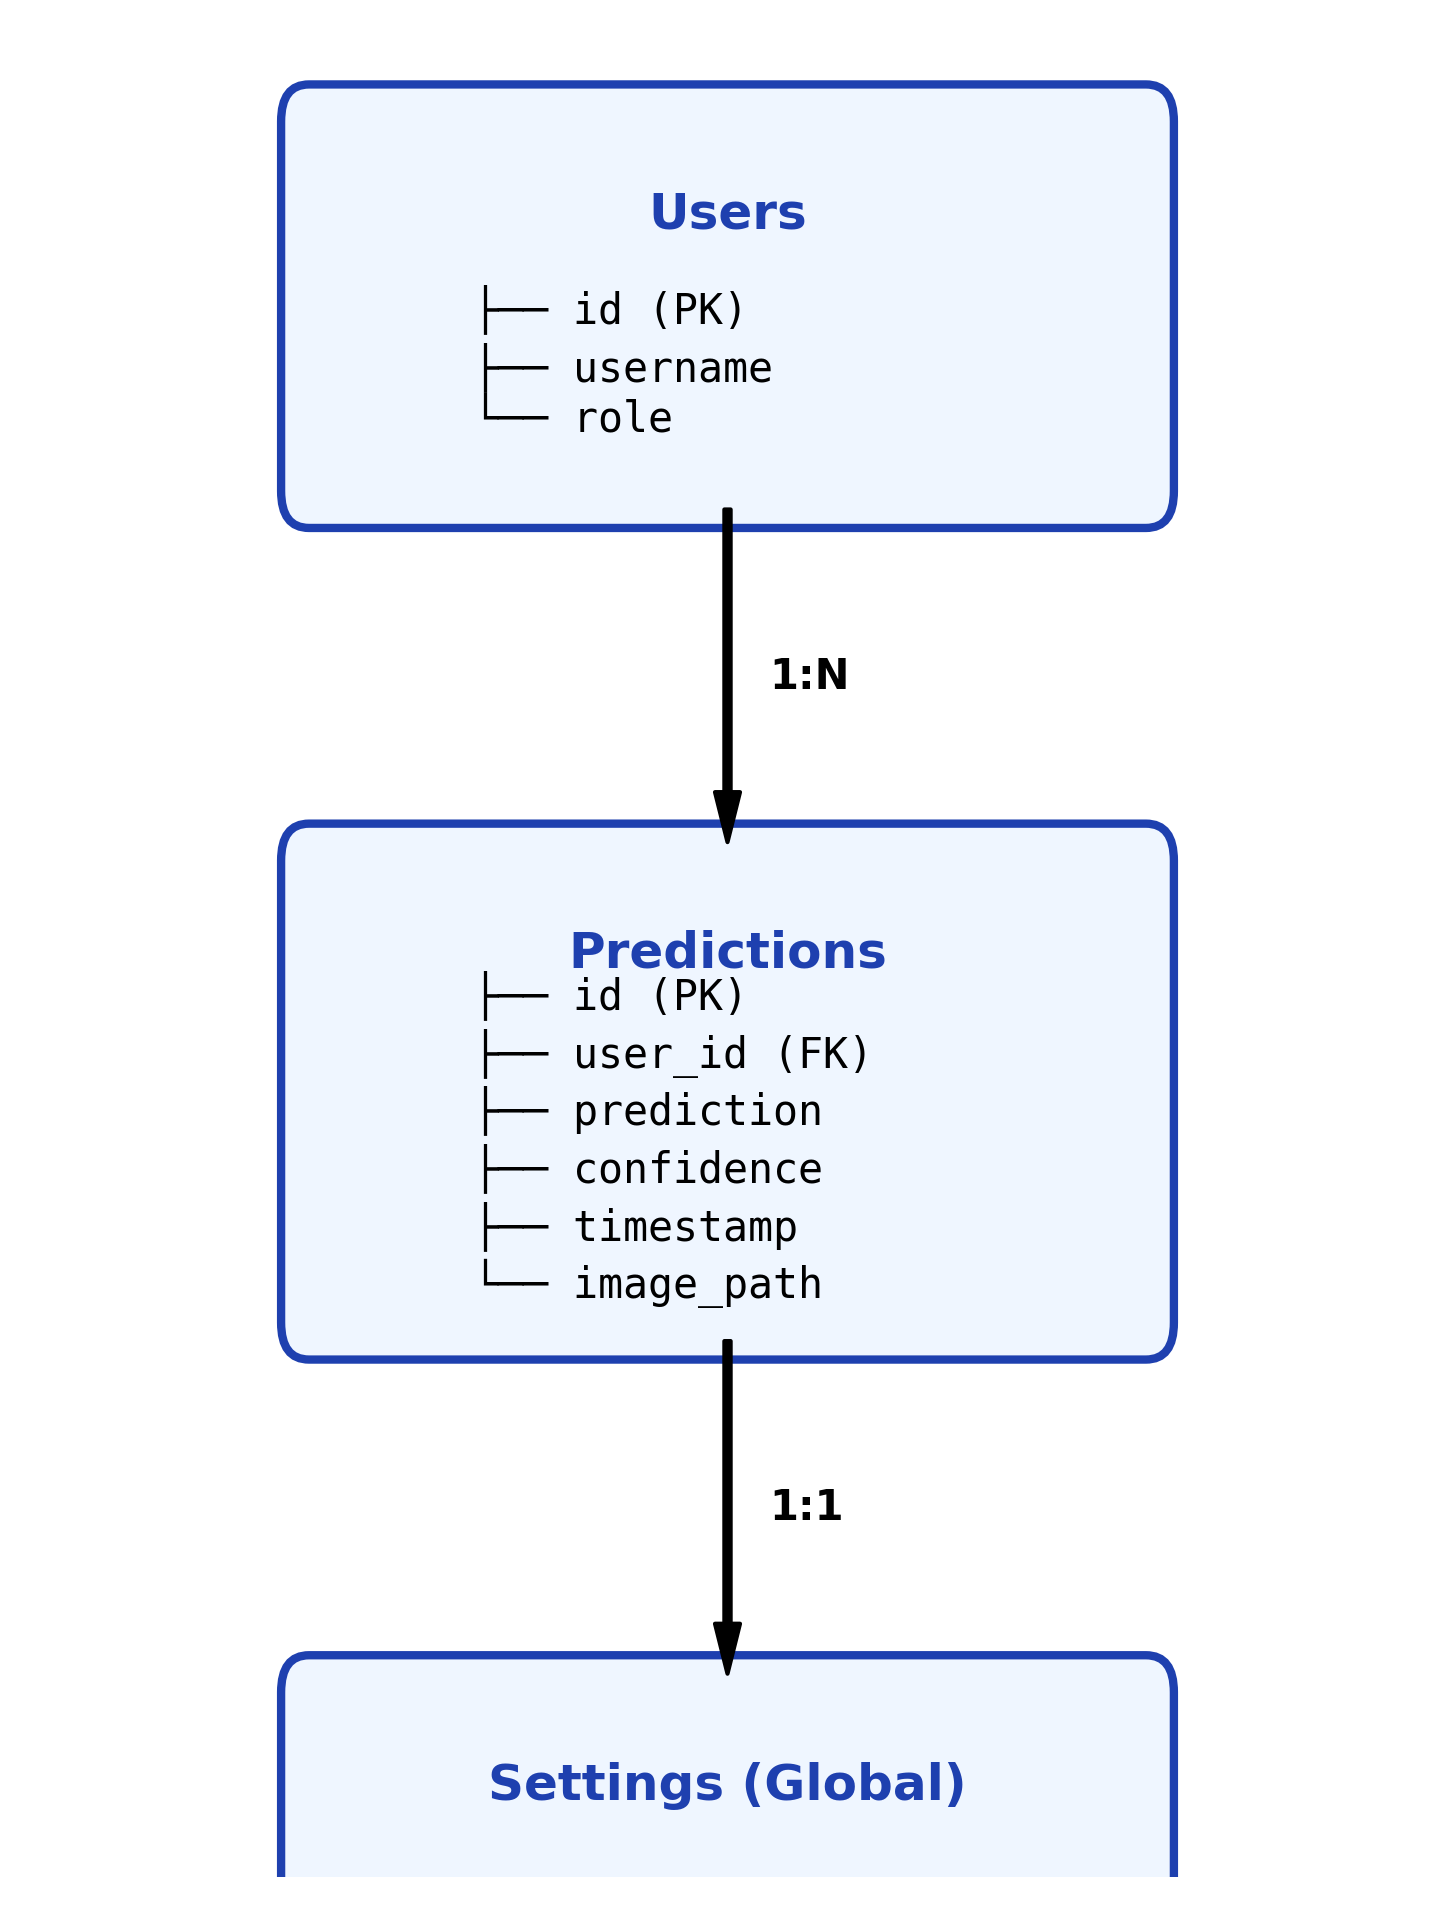
\includegraphics[width=0.8\textwidth]{images/er_diagram.png}
\caption{Entity Relationship (ER) Diagram}
\label{fig:er_diagram}
\end{figure}

\subsection{Frontend Dashboard}

A highly professional industrial dashboard was developed, heavily inspired by Google Stitch guidelines. The frontend features a responsive UI with a Dark Theme optimized for factory environments.

Modules included in the dashboard:
\begin{itemize}[leftmargin=1.5cm]
    \item \textbf{Executive Dashboard:} A high-level overview of daily statistics.
    \item \textbf{Inspection Module:} For manual image uploads and detailed analysis.
    \item \textbf{Live Monitoring:} To visualize real-time predictions.
    \item \textbf{Analytics:} Graphical representation of pass/fail trends.
    \item \textbf{Dataset Repository:} For managing training data.
    \item \textbf{Model Management \& Knowledge Center:} For administrative control and system documentation.
\end{itemize}

\begin{figure}[H]
\centering
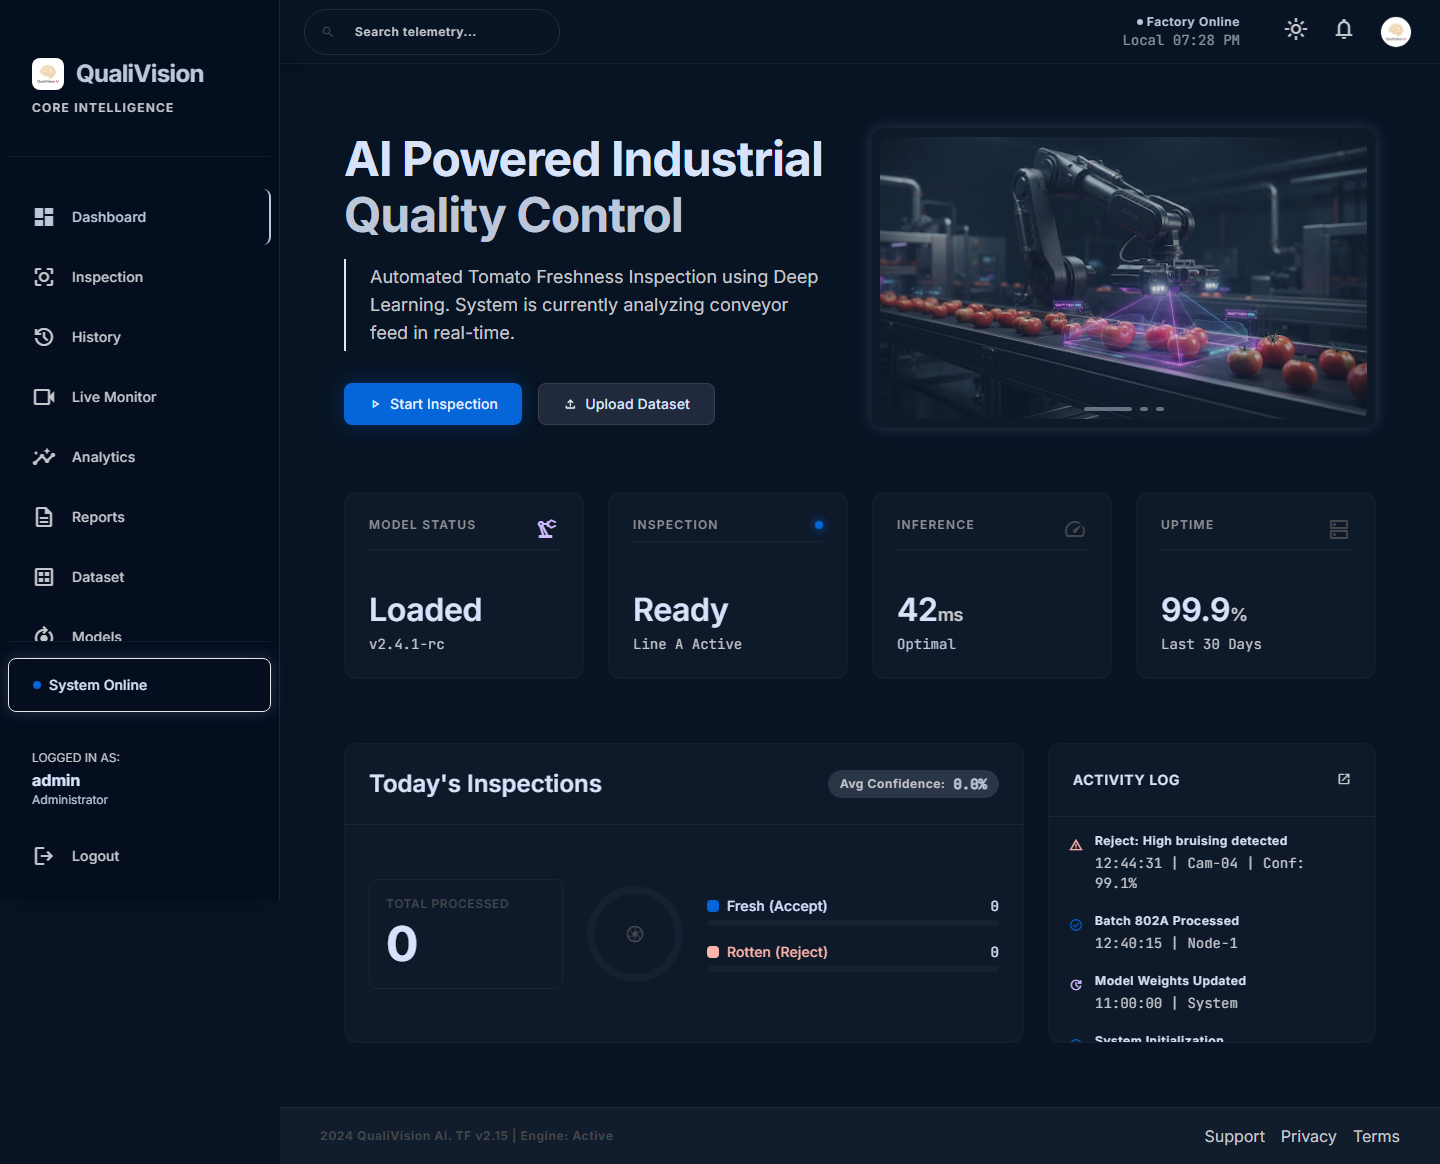
\includegraphics[width=0.8\textwidth]{images/02-dashboard.png}
\caption{QualiVision AI - Executive Dashboard}
\label{fig:dashboard}
\end{figure}

\begin{figure}[H]
\centering
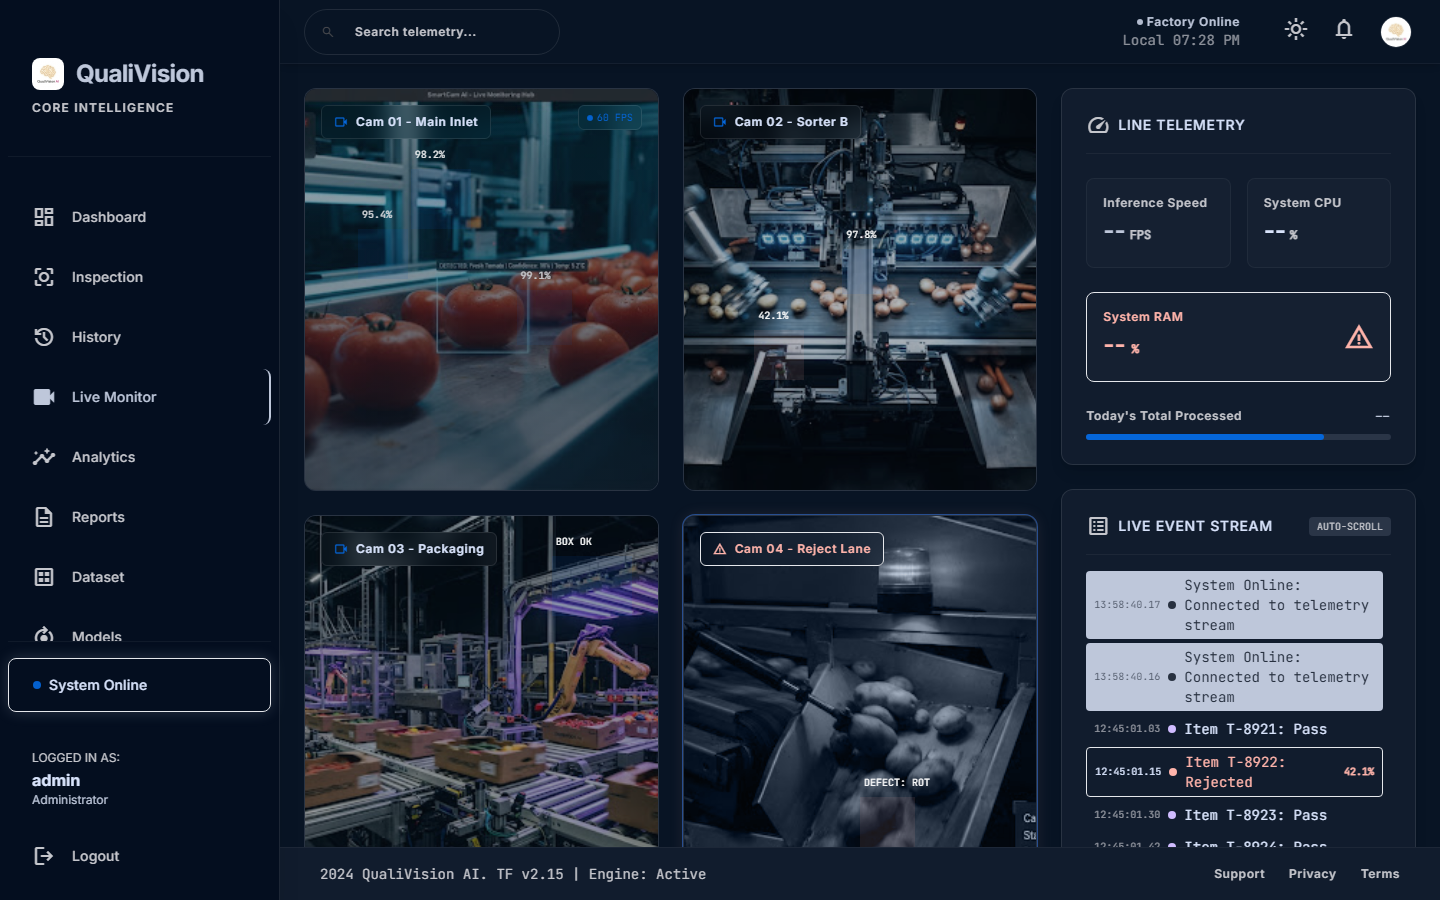
\includegraphics[width=0.8\textwidth]{images/03-live-monitoring.png}
\caption{QualiVision AI - Live Monitoring}
\label{fig:live_monitoring}
\end{figure}

\subsection{Testing and Results}

The system underwent exhaustive testing using fresh tomatoes, rotten tomatoes, unknown objects, and poor-quality images. The confidence threshold logic was validated to ensure that uncertain predictions were routed for manual review. Performance testing confirmed fast inference times and stable database operations.

The results demonstrated successful, real-time classification with high accuracy. The project proved that fast inference combined with an intuitive industrial dashboard provides substantial automation benefits.

\subsection{Future Scope and Conclusion}

Future improvements to the system could include Cloud Deployment, Edge AI optimizations, integration with IoT Cameras, Mobile App development, and migration to YOLO object detection for multi-object, real-time production line integration.

In conclusion, QualiVision AI represents a successful technical achievement, seamlessly integrating Computer Vision, Deep Learning, Flask Development, Database Management, and Dashboard Design. The project powerfully demonstrates how Artificial Intelligence can be practically deployed to solve complex Industrial Automation challenges.
